%
%     hw4_bbordwell.tex
%     Baylee Bordwell (baylee.bordwell@colorado.edu)
%     Based on the template by Benjamin Brown (bpbrown@colorado.edu)
%     Aug 27, 2014
%
%     Problem set 4 for ASTR/ATOC 5540, Mathematical Methods, taught at
%     University of Colorado, Boulder, Fall 2014.
%
%

\documentclass[10pt, preprint]{aastex}
% formatting based on 2014 NASA ATP proposal with Jeff Oishi

%%%%%%begin preamble
\usepackage[hmargin=1in, vmargin=1in]{geometry} % Margins
\usepackage{hyperref}
\usepackage{url}
\usepackage{times}
\usepackage{natbib}
\usepackage{graphicx}
\usepackage{amsmath}
\usepackage{amsfonts}
\usepackage{amssymb}
\usepackage{pdfpages}
\usepackage{import}
% for code import
\usepackage{listings}
\usepackage{color}
\usepackage{ragged2e}

\hypersetup{
     colorlinks   = true,
     citecolor     = gray,
     urlcolor       = blue
}

%% headers
\usepackage{fancyhdr}
\pagestyle{fancy}
\lhead{ASTR/ATOC 5540}
\chead{}
\rhead{name: Baylee Bordwell}
\lfoot{Problem Set 4}
\cfoot{\thepage}
\rfoot{Fall 2014}
% no hline under header
\renewcommand{\headrulewidth}{0pt}

\newcommand{\sol}{\ensuremath{\odot}}

% make lists compact
\usepackage{enumitem}
%\setlist{nosep}

%%%%%%end preamble


\begin{document}
\section*{Problem Set 4: Detrending Kepler Data}
\begin{enumerate}
\item It agrees!
\begin{figure}[!ht]  \centering
  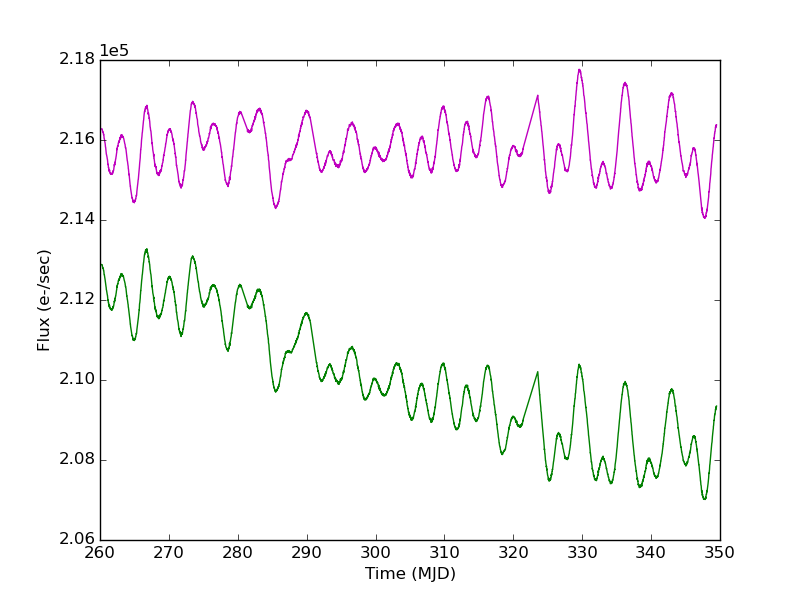
\includegraphics[width=4in]{hw4_fig1.png} %plot of lightcurve
\end{figure}

\item The fit becomes progressively better as $N$ increases, but even the linear solution is not terrible.
\begin{figure}[!ht]  \centering
  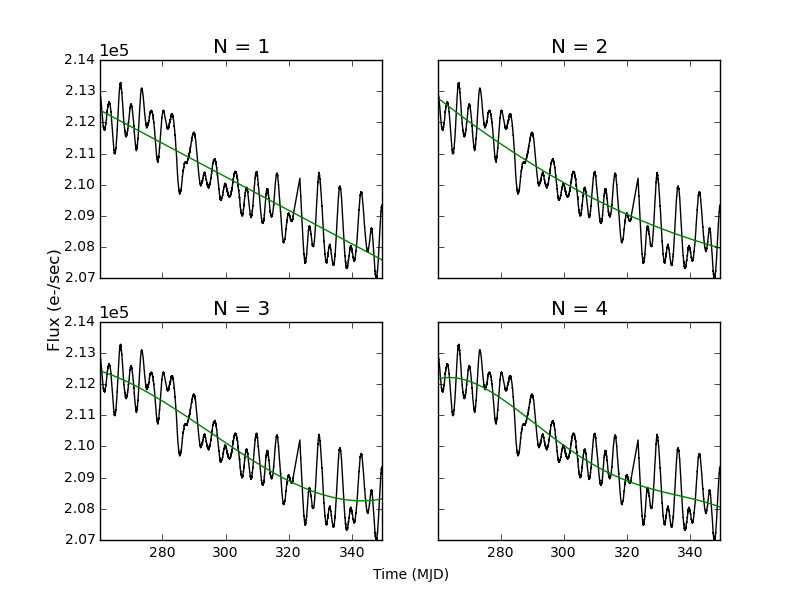
\includegraphics[width=5in]{hw4_fig2.png}
\end{figure}

\item As $N$ increases, the various metrics of error all decrease, until about $N = 5$, when the fit no longer significantly improves with $N$, and actually (around $N$ = 40) can go haywire and become terrible. This effect is due to precision errors and the conditioning number reaching the limits of double precision numbers' range.
\begin{figure}[!ht]  \centering
  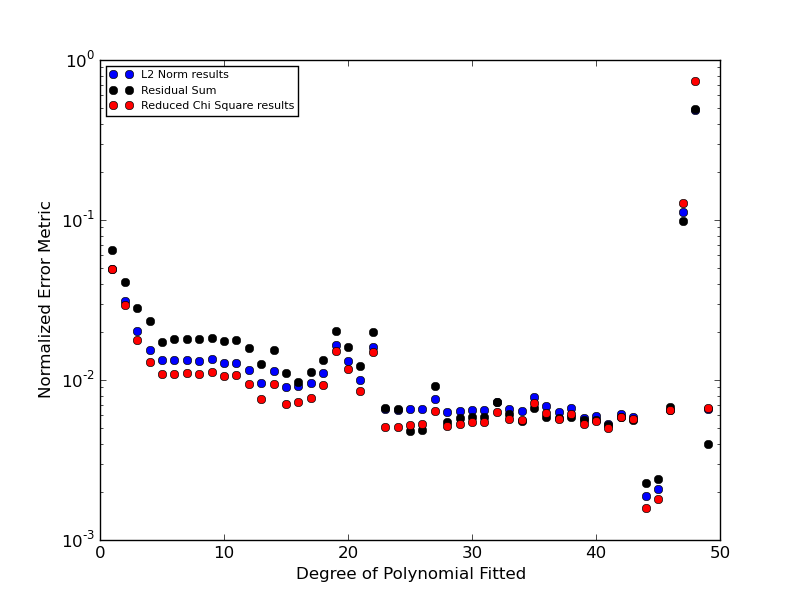
\includegraphics[width=5in]{hw4_fig3.png}
\end{figure}

\item  Only the polynomials up to $N=4$ in this solution make any significant difference to the final solution, therefore $N=4$ is a reasonable choice for detrending the data.
\begin{figure}[!ht]  \centering
  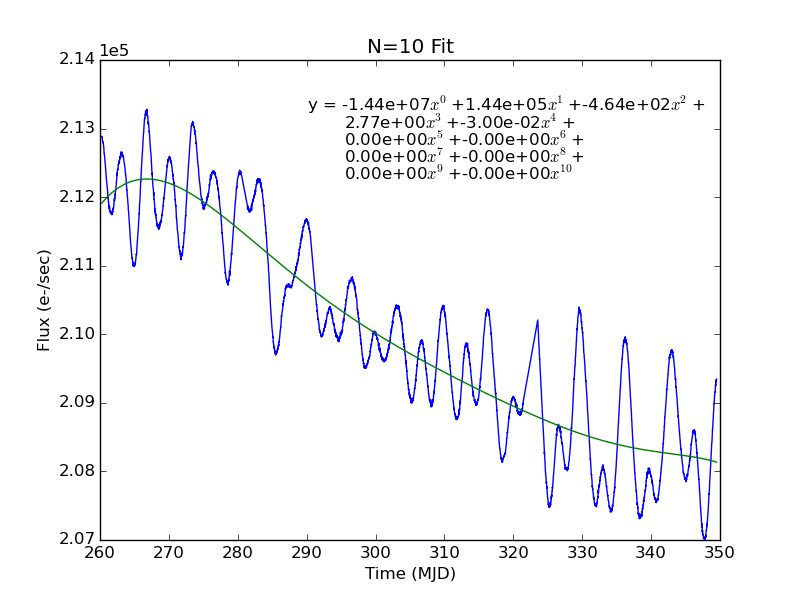
\includegraphics[width=5in]{hw4_fig4.png}
\end{figure}

\item Interestingly enough, if you choose a polynomial based purely on minimizing the L2 Norm, the sum of the residuals, or the reduced chi square, the ``best'' fit to detrend with would be $N=50$, which is plotted below and the L2 norm calculated to quantify the agreement with the PDC lightcurve.
\begin{figure}[!ht]  \centering
  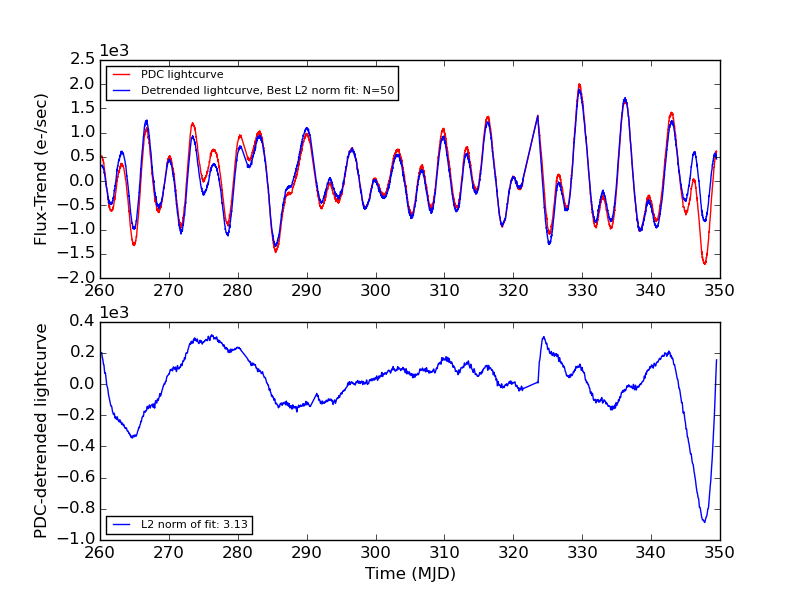
\includegraphics[width=5in]{hw4_fig5.png}
\end{figure}

If instead, following question 4, I were to choose $N=4$, I would find the following,
\begin{figure}[!ht]  \centering
  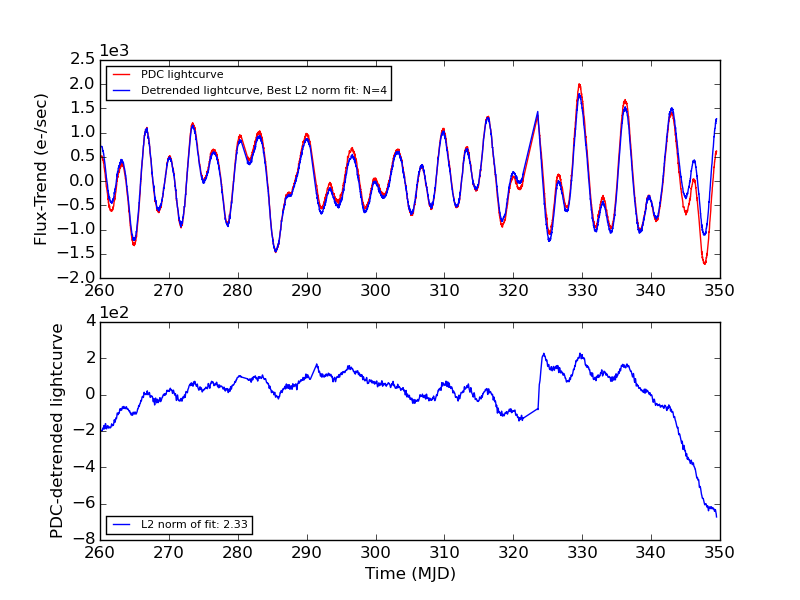
\includegraphics[width=5in]{hw4_fig6.png}
\end{figure}

And if I were to look at the smallest value of $N$ with good agreement (below), I would find that the smallest reasonable polynomial to use would be $N=3$, which is actually the best of them all.
\begin{figure}[!ht]  \centering
  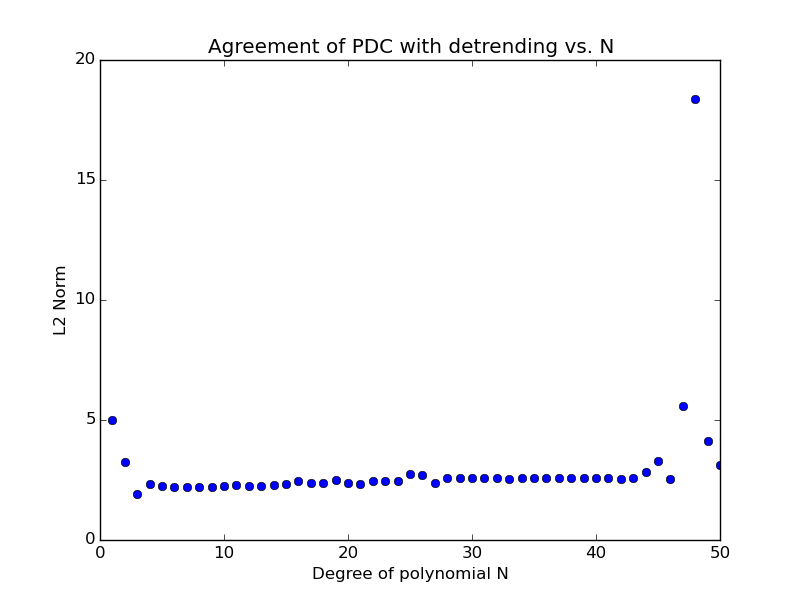
\includegraphics[width=5in]{hw4_fig7.png}
\end{figure}

\item The remaining wiggles in the stellar lightcurve are from a number of things. As this lightcurve was produced for a star with a possibly transiting exoplanet, some of the wiggles are from exoplanet transits, others may be from stellar activity such as pulsations and flares, and others from quasi-periodic variation due to stellar rotation, as well as good old fashioned noise (much smaller variations). The overall trend of our residual curve displays a mostly flat morphology with curvature towards the ends, which I would blame on fitting issues in dealing with the ends of a data set as well.

Given that this star does not display transits (at least according to the Kepler results so far), and that the wiggles are fairly stable and consistent, I would describe the large wiggling pattern as likely the result of observing a semi-regular variable star or RV Tauri. 

\end{enumerate}
\noindent Code involved in this assignment:
%
%     hw4_code.tex
%     Baylee Bordwell
%     Template from: Benjamin Brown (bpbrown@colorado.edu)
%     Aug 27, 2014
%
%     Problemset 4 for ASTR/ATOC 5540, Mathematical Methods, taught at
%     University of Colorado, Boulder, Fall 2014.
%
%     Python code importing block.
%


\definecolor{codegreen}{rgb}{0,0.6,0}
\definecolor{codegray}{rgb}{0.5,0.5,0.5}
\definecolor{codepurple}{rgb}{0.58,0,0.82}
\definecolor{backcolour}{rgb}{0.95,0.95,0.92}
 
\lstdefinestyle{mystyle}{
    backgroundcolor=\color{backcolour},   
    commentstyle=\color{codegreen},
    keywordstyle=\color{magenta},
    numberstyle=\tiny\color{codegray},
    stringstyle=\color{codepurple},
    basicstyle=\footnotesize,
    breakatwhitespace=false,         
    breaklines=true,                 
    captionpos=b,                    
    keepspaces=true,                 
    numbers=left,                    
    numbersep=5pt,                  
    showspaces=false,                
    showstringspaces=false,
    showtabs=false,                  
    tabsize=2
}

\lstset{style=mystyle}


\lstinputlisting[language=Python]{hw4_bbordwell.py}


\end{document}
